%\documentclass{beamer} % This is the file main.tex % ignore never use
%\documentclass[handout,aspectratio=169,mathserif,8pt,xcolor=table,notes=hide]{beamer}%iPad
%****************Handout*************
% \documentclass[handout,gray,xcolor=table]{beamer}
% \usepackage{pgfpages}
% \usepackage[8pt]{extsizes}
% \pgfpagesuselayout{2 on 1}[a4paper,border shrink=1mm]
%**************EndHandout*************
\documentclass[aspectratio=169,mathserif,8pt,xcolor=table,notes=show]{beamer}

%\usefonttheme{serif}
\usefonttheme[onlymath]{serif}%helps with readibility?
%\usetheme{Goettingen}
%\usetheme{Berlin} % Use for Review
\usetheme{CambridgeUS} % Use for lessons
\setbeamercolor{block title}{fg=gray!45!white,bg=darkred!80!black}
\setbeamercolor{frametitle}{fg=blue,bg=blue!20}
\setbeamerfont{section in head/foot}{size=\small} %make subsection font larger
\setbeamerfont*{subsection in head/foot}{size=\small} %make subsubsection font larger
\setbeamerfont{frametitle}{size=\tiny}
\setbeamertemplate{frametitle}{%
    \nointerlineskip%
    \begin{beamercolorbox}[wd=\paperwidth,ht=2.0ex,dp=0.6ex]{frametitle}
        \hspace*{1ex}\insertframetitle%
    \end{beamercolorbox}%
}%make frame title box smaller
%\usecolortheme{beaver}
%\usecolortheme{dolphin}
%\usecolortheme{lily}
%\usecolortheme{seahorse} %Use for Review
\usecolortheme{whale} %Use for lessons
\usepackage{color}
\usepackage{tikz}
\usepackage{multicol}%%%%TOC in two columns
\usepackage{ifthen}
\usepackage{animate}
\usepackage{multirow}
\usepackage{overpic}
%\usepackage[table,xcdraw]{xcolor}%Color in table
%\usepackage{enumitem}
\usepackage{pgfplots}
\usepackage{wrapfig}
%%%%MMC PACKAGES%%%%%%%%%
\usepackage{fancyvrb}
	\fvset{tabsize=4}%changes tab spacing in verbatim from 8 to 4
\usepackage{listings}
\definecolor{lightgrey}{rgb}{0.9,0.9,0.9}
\definecolor{darkgreen}{rgb}{0,0.6,0}

\lstset{language=[LaTeX]TeX,
texcsstyle=*\bf\color{blue},
numbers=none,
basicstyle=\small\ttfamily,
breaklines=true,
keywordstyle=\color{darkgreen},
commentstyle=\color{red},
%otherkeywords={$, \{, \}, \[, \]},
frame=none,
tabsize=2,
backgroundcolor=\color{lightgrey},
%caption=LaTeX example
}
\usepackage{epigraph}

\usetikzlibrary{patterns}%to shade rectangle


\title[Regression at MMC] %optional
{THE LINEAR REGRESSION PROCESS}}

\subtitle{From Generation to Interpretation}

\author[Briody] % (optional, for multiple authors)
{Frank Briody\\
\textit{frankbriody@gmail.com}  }


\institute[PHS] % (optional)
{
  Prospect High School\\
  Mt. Prospect, IL
}

\date[MMC 2022] % (optional)
{MMC Conference, February 2022}

%\logo{\includegraphics[height=1.5cm]{phs_logo.png}}

\begin{document}

	\begin{frame}
	\titlepage
	\end{frame}

% \section*{Outline}
% 	\begin{frame}
% 			\tableofcontents
% 	 \end{frame}
\section*{Outline}
	\begin{frame}
		\begin{multicols}{2}
			\tableofcontents
		\end{multicols}
	 \end{frame}
\AtBeginSection[]
{
 \begin{frame}<beamer>
  \begin{multicols}{2}
    \tableofcontents[currentsection,hideothersubsections]
    %\tableofcontents[currentsection]
  \end{multicols}
 \end{frame}
}


\section*{notes} % (fold)
\label{sec:notes}
	\note {
			}
% section notes (end)

\section{Prologue: Standard Deviation}

\begin{frame}[t]{}
How much variability, on average, is there around the mean?

%\includegraphics[width=.2\textwidth]{img/4_2_1}
%\includegraphics[width=.2\textwidth]{img/4_2_2}
%\includegraphics[width=.2\textwidth]{img/4_2_3}
%\includegraphics[width=.2\textwidth]{img/4_2_4}
%\includegraphics[width=.2\textwidth]{img/4_2_5}


\begin{table}[ht]
\large
%\centering
\huge{%
\begin{tabular*}{25cm}[h]{cccc}
Score & Deviation & Squared Deviation & \hspace{1.5in} \\
$x$ &  &  & \quad \\
\cline{1-4}
2 & \quad & \quad & \quad\\
4 & \quad & \quad & \\
6 & \quad & \quad & \\
8 & \quad & \quad & \\
15 & \quad & \quad &
\end{tabular*}
}
\end{table}
\end{frame}


\section{Pre-Installation} % (fold)
\label{sec:pre_installation}
	\subsection{What is LaTeX?} % (fold)
	\label{sub:what_is_latex_}
		\begin{frame}[fragile]{}
		\centering
		\Huge{\quad\\[.5in]What is \LaTeX ~?}
			\begin{columns}[]
				\begin{column}{.433\textwidth}
					\centering
					\epigraph{There is only one large computer program I have used in which there are to a decent approximation 0 bugs: Don Knuth's \TeX.}{\textit{ -- Jaap Weel}}
				\end{column}
				\begin{column}{.433\textwidth}
					\centering\quad\\[.5in]
					%\includegraphics[scale=.3]{ctan_lion_350x350.png}\\
				\end{column}
			\end{columns}
		\end{frame}
		\begin{frame}[fragile]{}
			\begin{columns}[T]
				\begin{column}{.433\textwidth}
					\centering
					\Huge{\quad\\[.5in]What\\[.2in] is\\[.2in] \LaTeX?}
				\end{column}
				\begin{column}{.433\textwidth}
					\centering\quad\\[.5in]
					%\includegraphics[scale=.3]{ctan_lion_350x350.png}\\
				\end{column}
			\end{columns}
			\begin{lstlisting}
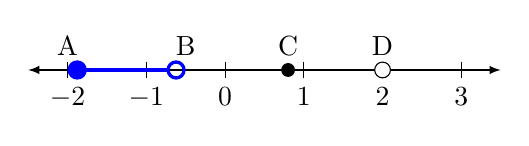
\begin{tikzpicture}[scale=1.0]
\usetikzlibrary{arrows}
  \draw[latex-latex] (-2.5,0) -- (3.5,0);
    \foreach \x in  {-2,-1,0,1,2,3}
      \draw[shift={(\x,0)},color=black] (0pt,3pt) -- (0pt,-3pt);
    \foreach \x in {-2,-1,0,1,2,3}
      \draw[shift={(\x,0)},color=black] (0pt,0pt) -- (0pt,-3pt) node[below] {$\x$};
    \draw[very thick,*-o,blue] (-2,0) -- (-.5,0);
    \node at (-2,.3) {A};
    \node at (-.5,.3) {B};
    \fill (0.8,0)  circle[radius=2.5pt];
    \node at (0.8,.3) {C};
    \draw[fill=white] (2,0) circle (.1cm);
    \node at (2,.3) {D};
\end{tikzpicture}

\end{lstlisting}
		\end{frame}
		{
		\setbeamercolor{background canvas}{bg=blue!40}
		\begin{frame}[plain]
			\centering
			%\includegraphics[width=.5\textwidth]{teacher.png}
		\end{frame}
		}
	% subsection what_is_latex_ (end)

	\subsection[Using \LaTeX ~Code]{Using LaTeX Inside Schoology, Google Docs, and Other Web-Based Applications} % (fold)
	\label{sub:using_latex_inside_schoology_google_docs_and_other_web_based_applications}
		\begin{frame}[fragile]
			\begin{columns}
				\begin{column}{6cm}
					\begin{lstlisting}
m=\frac{y_2-y_1}{x_2-x_1}
					\end{lstlisting}
					\quad\\[.5in]

					\begin{lstlisting}
x=\frac{-b\pm\sqrt{b^2-4ac}}{2a}
					\end{lstlisting}
				\end{column}
				\begin{column}{4cm}
				$m=\frac{y_2-y_1}{x_2-x_1}$\\[.5in]
				$x=\frac{-b\pm\sqrt{b^2-4ac}}{2a}$

				\end{column}
			\end{columns}
		\end{frame}

		\begin{frame}[t]{}
			\centering \Huge{Getting Help}\\
			%\includegraphics[scale=.2]{Google.png}\\
			\begin{columns}[T]
				\begin{column}{.5\textwidth}
					%\includegraphics[width=\textwidth]{StackExchange.png}\\
				\end{column}
				\begin{column}{.5\textwidth}
					%\includegraphics[width=\textwidth]{SE_Answer.png}\\
				\end{column}
			\end{columns}
		\end{frame}
	% subsection using_latex_inside_schoology_google_docs_and_other_web_based_applications (end)
% section pre_installation (end)

\section{Installation} % (fold)
\label{sec:installation}
	\subsection{Download and Install} % (fold)
		\label{sub:download_and_install}
		\begin{frame}[t]{}
		\centering {\Huge Getting and Starting}
			\begin{columns}[T]
				\begin{column}{.5\textwidth}
					\centering
					\quad\\[.2in]https://www.latex-project.org/get/\\[.2in]
					%\includegraphics[width=\textwidth]{Tex_Project.png}\\
					%\includegraphics[width=\textwidth]{Downloads.png}
				\end{column}
				\begin{column}{.5\textwidth}
					\centering
					\quad\\[.2in]
					Files\\[.2in]
					%\includegraphics[width=1\textwidth]{install.png}\\
				\end{column}
			\end{columns}
		\end{frame}
		% subsection download_and_install (end)
	\subsection{Using a Code Editor} % (fold)
		\label{sub:using_a_code_editor}
		\begin{frame}[t]{}
			\begin{columns}[T]
				\begin{column}{.433\textwidth}
					\centering
					TeXShop Code Editor\\[.1in]
					%\includegraphics[width=.5\textwidth]{Tex_Shop.png}\\[.1in]
					%\includegraphics[width=1.2\textwidth]{first_TexShop.png}\\
				\end{column}
				\begin{column}{.433\textwidth}
					\centering
					Output\\[.1in]
					%\includegraphics[width=1\textwidth]{first_Tex.pdf}\\[.2in]
					%\includegraphics[width=.8\textwidth]{aux_files.png}\\
				\end{column}
			\end{columns}
		\end{frame}
		% subsection using_a_code_editor (end)
	\subsection{Updating} % (fold)
		\label{sub:updating}
		\begin{frame}[t]{}
			\begin{columns}[T]
				\begin{column}{.2\textwidth}
				The TeXLive Utility\\[.1in]
					%\includegraphics[width=.8\textwidth]{TexLive.png}\\
				\end{column}
				\begin{column}{.8\textwidth}
					%\includegraphics[width=1\textwidth]{Updates.png}\\
				\end{column}
			\end{columns}
		\end{frame}
		% subsection updating (end)
	\subsection{Optional Installations} % (fold)
		\label{sub:optional_installations}
		\begin{frame}[t]{}
			\centering
			\begin{columns}[T]
				\begin{column}{.333\textwidth}
					\centering
					Skim pdf viewer\\ free\\[.1in]
					%\includegraphics[width=\textwidth]{Skim.png}
				\end{column}
				\begin{column}{.333\textwidth}
					\centering
					Sublime Text 3 code editor\\ \$80 donationware\\[.1in]
					%\includegraphics[width=\textwidth]{SublimeText.png}
				\end{column}
				\begin{column}{.333\textwidth}
					\centering
					Text Expander\\ about \$28/year education\\[.1in]
					%\includegraphics[width=\textwidth]{TextExpander.png}
				\end{column}
			\end{columns}
		\end{frame}
		% subsection optional_installations (end)
% section installation (end)

\section{Diagrams and Graphs} % (fold)
\label{sec:diagrams_and_graphs}
	\subsection{Blank Grids} % (fold)
		\label{sub:blank_grids}
		\subsubsection{Number Line}
			\begin{frame}[fragile]
				\centering
				{\Huge Number Line}\\[.2in]
				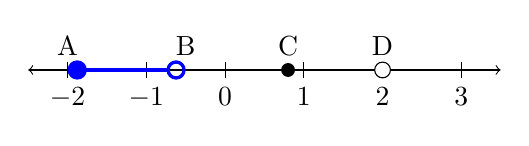
\begin{tikzpicture}[scale=1]
						\usetikzlibrary{arrows}
						\draw[<->] (-2.5,0) -- (3.5,0); %edit here for the axis
						% \foreach \x in  {-2,-1,0,1,2,3} % edit here for the vertical lines
						% \draw[shift={(\x,0)},color=black] (0pt,3pt) -- (0pt,-3pt);
						\foreach \x in {-2,-1,0,1,2,3} % edit here for the numbers
						\draw[shift={(\x,0)},color=black] (0pt,3pt) -- (0pt,-3pt) node[below]
						{$\x$};
						\draw[very thick,*-o,blue] (-2,0) -- (-.5,0);
						\node at (-2,.3) {A};
						\node at (-.5,.3) {B};
						\fill (0.8,0)  circle[radius=2.5pt];
						\node at (0.8,.3) {C};
						\draw[fill=white] (2,0) circle (.1cm);
						\node at (2,.3) {D};
				\end{tikzpicture}\\

				\begin{lstlisting}
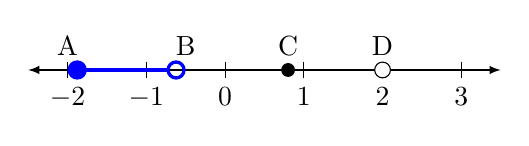
\begin{tikzpicture}[scale=1.0]
\usetikzlibrary{arrows}
   \draw[latex-latex] (-2.5,0) -- (3.5,0);
    \foreach \x in {-2,-1,0,1,2,3}
      \draw[shift={(\x,0)},color=black] (0pt,3pt) -- (0pt,-3pt) node[below] {$\x$};
    \draw[very thick,*-o,blue] (-2,0) -- (-.5,0);
    \node at (-2,.3) {A};
    \node at (-.5,.3) {B};
    \fill (0.8,0)  circle[radius=2.5pt];
    \node at (0.8,.3) {C};
    \draw[fill=white] (2,0) circle (.1cm);
    \node at (2,.3) {D};
\end{tikzpicture}
				\end{lstlisting}
			\end{frame}

		\subsubsection{Cartesian Plane}
			\begin{frame}[fragile]
				\centering
				{\Huge Cartesian Plane}\\[.2in]
				\begin{columns}[T]
					\begin{column}{.75\textwidth}
						\begin{lstlisting}
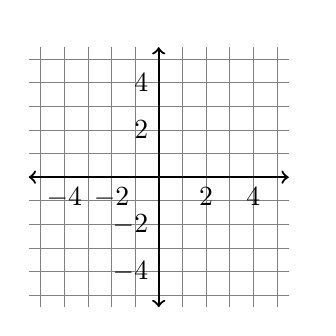
\begin{tikzpicture}[xscale=.3,yscale=.3]
	\draw[style = help lines, step=1cm] (-5.5,-5.5) grid (5.5,5.5);
	 \draw[thick,<->] (-5.5,0) -- (5.5,0) node[anchor=north west] {};
	 \draw[thick,<->] (0,-5.5) -- (0,5.5) node[anchor=south east] {};
	 \foreach \x in {-4,-2,2,4}
	 	\draw (\x cm,1pt) -- (\x cm,-1pt) node[anchor=north] {$\x$};
	 \foreach \y in {-4, -2, 2,4}
	 	\draw (1pt,\y cm) -- (-1pt,\y cm) node[anchor=east] {$\y$};
\end{tikzpicture}
				\end{lstlisting}
					\end{column}
					\begin{column}{.25\textwidth}
						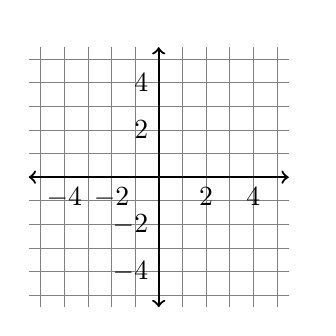
\begin{tikzpicture}[xscale=.3,yscale=.3]%[y=1cm,x=1cm]
	\draw[style = help lines, step=1cm] (-5.5,-5.5) grid (5.5,5.5);
	 \draw[thick,<->] (-5.5,0) -- (5.5,0) node[anchor=north west] {};%{x};
	 \draw[thick,<->] (0,-5.5) -- (0,5.5) node[anchor=south east] {};%{y};
	 \foreach \x in {-4,-2,2,4}
	 \draw (\x cm,1pt) -- (\x cm,-1pt) node[anchor=north] {$\x$};
	 \foreach \y in {-4, -2, 2,4}
	 \draw (1pt,\y cm) -- (-1pt,\y cm) node[anchor=east] {$\y$};
\end{tikzpicture}
					\end{column}
				\end{columns}
			\end{frame}
		% subsection blank_grids (end)
	\subsection{Functions} % (fold)
		\label{sub:functions}
		\subsubsection{Basic}
			\begin{frame}[fragile]
			\centering
				{\Huge Function with Point}\\[.2in]
				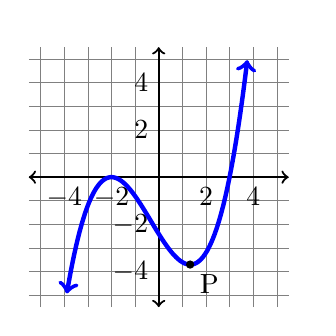
\begin{tikzpicture}[xscale=.3,yscale=.3]%[y=1cm,x=1cm]
				\draw[style = help lines, step=1cm] (-5.5,-5.5) grid (5.5,5.5);
				 \draw[thick,<->] (-5.5,0) -- (5.5,0) node[anchor=north west] {};%{x};
				 \draw[thick,<->] (0,-5.5) -- (0,5.5) node[anchor=south east] {};%{y};
				 \foreach \x in {-4,-2,2,4}
				 \draw (\x cm,1pt) -- (\x cm,-1pt) node[anchor=north] {$\x$};
				 \foreach \y in {-4, -2, 2,4}
				 \draw (1pt,\y cm) -- (-1pt,\y cm) node[anchor=east] {$\y$};
				 \draw[ultra thick,blue,<->] plot[domain=-3.89:3.75,samples=100] (\x,{.2*(\x+2)^2*(\x-3)});
				 \fill (1.33,-3.7)  circle[radius=5pt] node[anchor=north west]{P};
         	\end{tikzpicture}\\
			\begin{lstlisting}
\draw[ultra thick,blue,<->] plot[domain=-3.89:3.75,samples=100] (\x,{.2*(\x+2)^2*(\x-3)});
\fill (1.33,-3.7)  circle[radius=5pt] node[anchor=north west]{P};
			\end{lstlisting}
		\end{frame}
		\begin{frame}[fragile]
			\centering
				{\Huge Points, Dashed Line and Piecewise}\\[.1in]
				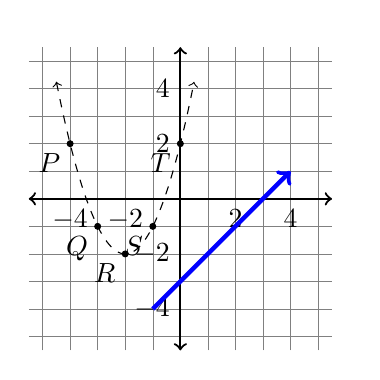
\begin{tikzpicture}[xscale=.35,yscale=.35]%[y=1cm,x=1cm]
					\usetikzlibrary{arrows}
					\draw[style = help lines, step=1cm] (-5.5,-5.5) grid (5.5,5.5);
					 \draw[thick,<->] (-5.5,0) -- (5.5,0) node[anchor=north west] {};%{x};
					 \draw[thick,<->] (0,-5.5) -- (0,5.5) node[anchor=south east] {};%{y};
					 \foreach \x in {-4,-2,2,4}
					 	\draw (\x cm,1pt) -- (\x cm,-1pt) node[anchor=north] {$\x$};
					 \foreach \y in {-4, -2, 2,4}
					 	\draw (1pt,\y cm) -- (-1pt,\y cm) node[anchor=east] {$\y$};
					 \draw[->,ultra thick,blue] (-1,-4) -- (4,1);
		            \foreach\x/\y/\z in {-4/2/P,-3/-1/Q,-2/-2/R,-1/-1/S,0/2/T}
		                \draw [fill=black] (\x,\y)circle (3pt) node[below left] {$\z$};
		            \draw[dashed,<->] plot[domain=-4.5:0.5,samples=100] (\x,{(\x+2)^2-2)});
		         \end{tikzpicture}
			\begin{lstlisting}
\foreach\x/\y/\z in {-4/2/P,-3/-1/Q,-2/-2/R,-1/-1/S,0/2/T}
     \draw [fill=black] (\x,\y)circle (3pt) node[below left] {\z};
\draw[dashed,<->] plot[domain=-4.5:0.5,samples=100] (\x,{(\x+2)^2-2)});
\draw[->,ultra thick,blue] (-1,-4) -- (4,1);
			\end{lstlisting}
		\end{frame}
		\subsubsection{Scale}
			\begin{frame}[fragile]
				\begin{columns}[T]
					\begin{column}{.5\textwidth}
						\centering
						\quad\\[.5in]
						{\Huge Changing Scale}\\[.2in]
					\end{column}
					\begin{column}{.5\textwidth}
						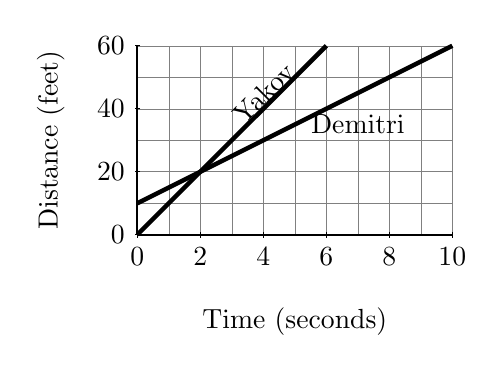
\begin{tikzpicture}[y=.04cm, x=.4cm]
						\draw[style=help lines, ystep=10, xstep=1] (0,0) grid (10,60);
						\draw[thick,-] (0,0) -- coordinate (x axis mid) (10,0);
						\draw[thick,-] (0,0) -- coordinate (y axis mid) (0,60);
						\foreach \x in {0,2,4,6,8,10}
						    \draw (\x ,1pt) -- (\x ,-1pt) node[anchor=north] {$\x$};
						\foreach \y in {0,20,40,60}
						    \draw (1pt,\y ) -- (-1pt,\y ) node[anchor=east] {$\y$};
						\draw[-, ultra thick, domain=-0:6,smooth] plot (\x, {10*\x});
						\node[rotate=45] at (4,45) {Yakov};
						\node[rotate=0] at (7,35) {Demitri};
						\draw[-, ultra thick, domain=-0:10,smooth] plot (\x, {5*\x+10});
						\node[below=0.8cm] at (x axis mid) {Time (seconds)};
						\node[rotate=90, above=0.8cm] at (y axis mid) {Distance (feet)};
						\end{tikzpicture}
					\end{column}
				\end{columns}
				\begin{lstlisting}
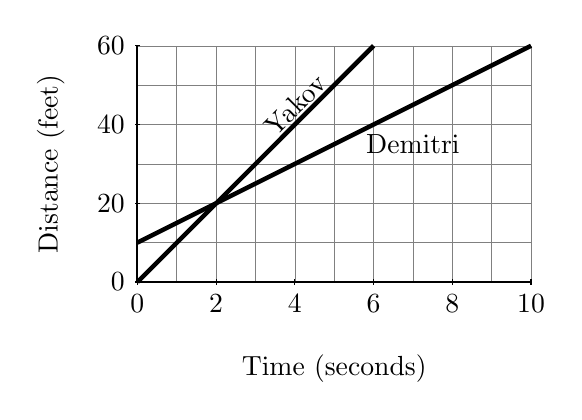
\begin{tikzpicture}[y=.05cm, x=.5cm]
    \draw[style=help lines, ystep=10, xstep=1] (0,0) grid (10,60);
    \draw[thick,-] (0,0) -- coordinate (x axis mid) (10,0);
    \draw[thick,-] (0,0) -- coordinate (y axis mid) (0,60);
    \foreach \x in {0,2,4,6,8,10}
        \draw (\x ,1pt) -- (\x ,-1pt) node[anchor=north] {$\x$};
    \foreach \y in {0,20,40,60}
        \draw (1pt,\y ) -- (-1pt,\y ) node[anchor=east] {$\y$};
    \draw[-, ultra thick, domain=-0:6,smooth] plot (\x, {10*\x});
    \node[rotate=45] at (4,45) {Yakov};
    \node[rotate=0] at (7,35) {Demitri};
    \draw[-, ultra thick, domain=-0:10,smooth] plot (\x, {5*\x+10});
    \node[below=0.8cm] at (x axis mid) {Time (seconds)};
    \node[rotate=90, above=0.8cm] at (y axis mid) {Distance (feet)};
\end{tikzpicture}\\
					\end{lstlisting}
			\end{frame}

		\subsubsection{Domain}
			\begin{frame}[fragile]
				\begin{columns}[T]
					\begin{column}{.433\textwidth}
						\centering
						\quad\\[.5in]
						{\Huge Rational Function}\\[.2in]
					\end{column}
					\begin{column}{.433\textwidth}
						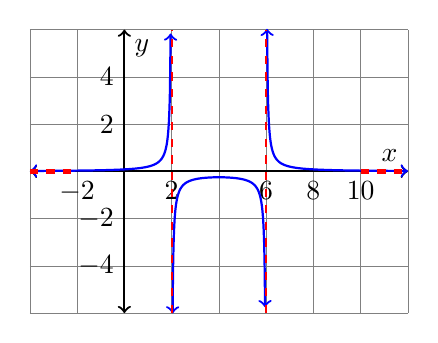
\begin{tikzpicture}[scale=.3]\label{caption_ex}
							\draw[style=help lines, ystep=2, xstep=2] (-4,-6) grid (12,6);%grid
							\draw[thick,<->] (-4,0) -- (12,0) node[anchor=south east] {$x$};
							\draw[thick,<->] (0,-6) -- (0,6) node[anchor=north west] {$y$};
							\foreach \x in {-2,2,6,8,10}
							    \draw (\x cm,1pt) -- (\x cm,-1pt) node[anchor=north] {$\x$};
							\foreach \y in {-4,-2,2,4}
							    \draw (1pt,\y cm) -- (-1pt,\y cm) node[anchor=east] {$\y$};
							%\draw[<->, ultra thick, domain=0:8,smooth] plot (\x, {\x*\x-8*\x+12});
							\draw[blue,<->, thick, domain=-4:1.959,smooth,samples=200] plot (\x, {1/(\x*\x-8*\x+12)});
							\draw[blue,<->, thick, domain=2.042:5.958,smooth,samples=200] plot (\x, {1/(\x*\x-8*\x+12)});
							\draw[blue,<->, thick, domain=6.041:12,smooth,samples=200] plot (\x, {1/(\x*\x-8*\x+12)});
							\draw[red,thick,dashed] (2,-6) -- (2,6);%Vert Asymp
							\draw[red,thick,dashed] (6,-6) -- (6,6);%Vert Asymp
							\draw[red,ultra thick,dashed] (-4,0) -- (-2,0);%Horiz Asymp
							\draw[red,ultra thick,dashed] (10,0) -- (12,0);%Horiz Asymp
						\end{tikzpicture}
					\end{column}
				\end{columns}
				\begin{lstlisting}
\draw[blue,<->, thick, domain=-4:1.959,smooth,samples=200] plot (\x, {1/(\x*\x-8*\x+12)});
\draw[blue,<->, thick, domain=2.042:5.958,smooth,samples=200] plot (\x, {1/(\x*\x-8*\x+12)});
\draw[blue,<->, thick, domain=6.041:12,smooth,samples=200] plot (\x, {1/(\x*\x-8*\x+12)});
\draw[red,thick,dashed] (2,-6) -- (2,6);%Vert Asymp
\draw[red,thick,dashed] (6,-6) -- (6,6);%Vert Asymp
\draw[red,ultra thick,dashed] (-4,0) -- (-2,0);%Horiz Asymp
\draw[red,ultra thick,dashed] (10,0) -- (12,0);%Horiz Asymp
				\end{lstlisting}
			\end{frame}
		\subsubsection{Drawing}
		\begin{frame}[fragile]
			\begin{columns}[T]
				\begin{column}{.4\textwidth}
					\centering
						\quad\\[.5in]
						{\Huge Drawing Curves}\\[.2in]
				\end{column}
				\begin{column}{.6\textwidth}
					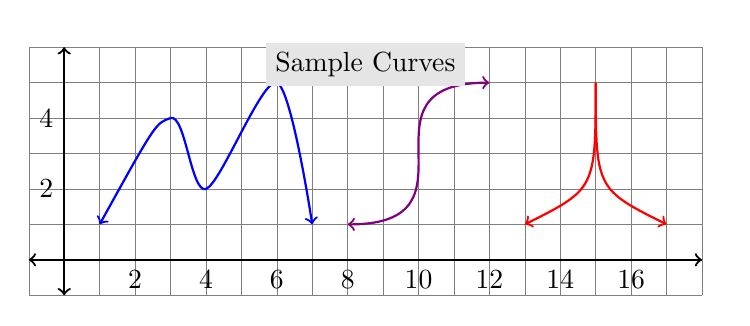
\begin{tikzpicture}[xscale=.45,yscale=.45]\label{node_ex}%[y=1cm,x=1cm]
            \draw[style = help lines, step=1cm] (-1,-1) grid (18,6);
            \foreach \x in {2,4,6,8,10,12,14,16}
	            \draw (\x cm,1pt) -- (\x cm,-1pt) node[anchor=north] {$\x$};
            \foreach \y in {2,4}
               \draw (1pt,\y cm) -- (-1pt,\y cm) node[anchor=east] {$\y$};
            \draw[thick,<->] (-1,0) -- (18,0) node[anchor=north west] {};%{x};
            \draw[thick,<->] (0,-1) -- (0,6) node[anchor=south east] {};%{y};
			\draw[blue,<->,thick] plot [smooth] coordinates {(1,1) (3,4) (4,2) (6,5) (7,1)};
			\draw[violet, thick,<->] (8,1) .. controls (12,1) and (8,5) .. (12,5);
			\draw[red, thick,<-] (13,1) .. controls (15,2) .. (15,5);
			\draw[red, thick,->] (15,5) .. controls (15,2) .. (17,1);
			\node[fill=black!10] at (8.5,5.5) {Sample Curves};
        \end{tikzpicture}
				\end{column}
			\end{columns}
			\begin{lstlisting}
\draw[blue,<->,thick] plot [smooth] coordinates {(1,1) (3,4) (4,2) (6,5) (7,1)};
\draw[violet, thick,<->] (8,1) .. controls (12,1) and (8,5) .. (12,5);
\draw[red, thick,<-] (13,1) .. controls (15,2) .. (15,5);
\draw[red, thick,->] (15,5) .. controls (15,2) .. (17,1);
\node[fill=black!10] at (8.5,5.5) {Sample Curves};
				\end{lstlisting}
		\end{frame}


		\subsubsection{Legend}
				\begin{frame}[fragile]
			\begin{columns}[T]
				\begin{column}{.433\textwidth}
					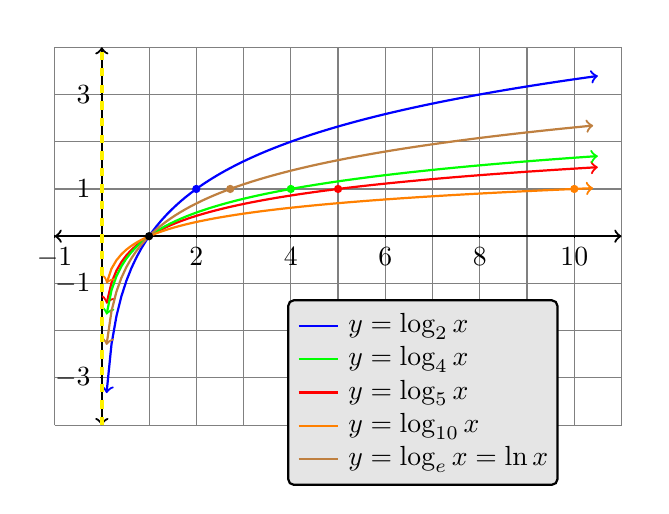
\begin{tikzpicture}[scale=.6]
						\draw[step=1cm,gray, thin] (-1,-4) grid (11,4);
						\draw[thick,<->] (-1,0) -- (11,0) node[anchor=north west] {};%{x};
						\draw[thick,<->] (0,-4) -- (0,4) node[anchor=south east] {};%{y};
						\foreach \x in {-1,2,4, 6, 8, 10}
						\draw (\x cm,1pt) -- (\x cm,-1pt) node[anchor=north] {$\x$};
						\foreach \y in {-1,-3,1,3}
						\draw (1pt,\y cm) -- (-1pt,\y cm) node[anchor=east] {$\y$};
						\draw[<->,thick,blue] plot[domain=0.1:10.5,samples=100] (\x,{log2(\x)});
						\draw[<->,thick,red] plot[domain=0.1:10.5,samples=100] (\x,{(log2(\x))/(log2(5))});
						\draw[<->,thick,green] plot[domain=0.1:10.5,samples=100] (\x,{(log2(\x))/(log2(4))});
						\draw[<->,thick,orange] plot[domain=0.1:10.4,samples=100] (\x,{(log2(\x))/(log2(10))});
						\draw[<->,thick,brown] plot[domain=0.1:10.4,samples=100] (\x,{(log2(\x))/(log2(2.718))});
						\draw[ultra thick, dashed,yellow] (0,-4)--(0,4);
						\fill (1,0) circle[radius=2.5pt];
						\fill[blue] (2,1) circle[radius=2.5pt];
						\fill[red] (5,1) circle[radius=2.5pt];
						\fill[green] (4,1) circle[radius=2.5pt];
						\fill[orange] (10,1) circle[radius=2.5pt];
						\fill[brown] (2.71828,1) circle[radius=2.5pt];
						%\node[draw=black,thick,fill=white,rounded corners=2pt,below left=2mm] at (3.6,4.2) {%
						\node[draw=black,thick,fill=black!10,rounded corners=2pt,below left=2mm] at (10,-1) {%
						\begin{tabular}{@{}r@{ }l@{}}
						 \raisebox{2pt}{\tikz{\draw[thick,blue] (0,0) -- (5mm,0);}}&$y=\log_2 x$\\
						 \raisebox{2pt}{\tikz{\draw[thick,green] (0,0) -- (5mm,0);}}&$y=\log_4 x$\\
						 \raisebox{2pt}{\tikz{\draw[thick,red] (0,0) -- (5mm,0);}}&$y=\log_5 x$\\
						 \raisebox{2pt}{\tikz{\draw[thick,orange] (0,0) -- (5mm,0);}}&$y=\log_{10} x$\\
						 \raisebox{2pt}{\tikz{\draw[thick,brown] (0,0) -- (5mm,0);}}&$y=\log_{e} x=\ln x$
						\end{tabular}};
					\end{tikzpicture}
				\end{column}
				\begin{column}{.433\textwidth}
					\centering
						\quad\\[.5in]
						{\Huge Adding a Legend}\\[.2in]
						\&\\[.2in]
						\href{http://www.texample.net/tikz/examples/}{\beamergotobutton{{\normalsize The TIKZ Gallery of Examples}}}
				\end{column}
			\end{columns}
			\begin{lstlisting}
\node[draw=black,thick,fill=black!10,rounded corners=2pt,below left=2mm] at (10,-1) {%
\begin{tabular}{@{}r@{ }l@{}}
 \raisebox{2pt}{\tikz{\draw[thick,blue] (0,0) -- (5mm,0);}}&$y=\log_2 x$\\
 \raisebox{2pt}{\tikz{\draw[thick,green] (0,0) -- (5mm,0);}}&$y=\log_4 x$\\
 \raisebox{2pt}{\tikz{\draw[thick,red] (0,0) -- (5mm,0);}}&$y=\log_5 x$\\
 \raisebox{2pt}{\tikz{\draw[thick,orange] (0,0) -- (5mm,0);}}&$y=\log_{10} x$\\
 \raisebox{2pt}{\tikz{\draw[thick,brown] (0,0) -- (5mm,0);}}&$y=\log_{e} x=\ln x$
\end{tabular}};
			\end{lstlisting}
		\end{frame}

		\subsubsection{Gallery}

		% subsection functions (end)
	\subsection{Diagrams} % (fold)
		\label{sub:diagrams}
		\begin{frame}[fragile]
			\begin{columns}[T]
				\begin{column}{.433\textwidth}
					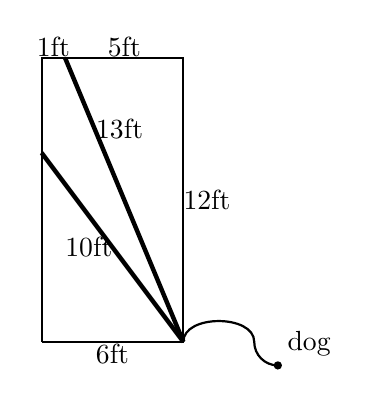
\begin{tikzpicture}[scale=.3]
						%\draw[gray] (0,-2) grid (10,12);
						\draw[  thick,-] (0,0) -- (6,0) -- (6,12)--(0,12)--(0,0);%node[anchor=north east] {m};
						\draw[ultra thick,-] (6,0)--(0,8);
						\draw[ultra thick,-] (6,0)--(1,12);
						%\node[anchor=north east] {m};
						\node at (.5,12.5) {1ft};
						\node at (3.5,12.5) {5ft};
						\node at (7,6) {12ft};
						\node at (3,-.5) {6ft};
						\node at (3.3,9) {13ft};
						\node at (2,4) {10ft};
						\fill (10,-1)  circle[radius=5pt] node[anchor=south west]  {dog};
						\draw [-,thick] (6,0) [out=90 ,in=90] to (9,0) [out=270 ,in=180 ] to (10,-1);
						\end{tikzpicture}\\
					\begin{lstlisting}
%\draw[gray] (0,-2) grid (10,12);

\draw [-,thick] (6,0) [out=90 ,in=90] to (9,0) [out=270 ,in=180 ] to (10,-1);
					\end{lstlisting}
				\end{column}
				\begin{column}{.433\textwidth}
					\usetikzlibrary{calc}
		            \newcommand\irregularline[2]{%
		                let \n1 = {rand*(#1)} in
		                +(0,\n1)
		                \foreach \a in {0.1,0.2,...,#2}{
		                let \n1 = {rand*(#1)} in
		                -- +(\a,\n1)
		                    }
		            }
		 			\begin{tikzpicture}[scale=.5]
		            \draw[thick,blue] (-6,4) \irregularline{0.1cm}{12};
		            \fill[gray,opacity=.5] (-6,0) rectangle (6,4);
		            \draw[|-|] (-5,0)--(-5,4) node [midway] {6ft};
		            \draw[thick,dashed] (-4,0)--(-4,4);
		            \draw[<-,ultra thick,dashed] (-4,0)--(-1,4);
		            \draw[<-,ultra thick,dashed] (-1,4.2)--(5,4.2);
		            \draw[|-|] (-4,6)--(5,6) node [midway,fill=white] {20ft};
		            \node[anchor=south] at (-4,4) {$O$};
		            \node[anchor=north west] at (-4,0) {$B$};
		            \node[anchor=north west] at (-1,4) {$S$};
		            \node[anchor=north west] at (5,4) {$M$};
		            \draw[fill=black] (-4,0) circle (5pt);%CLOSED CIRCLE
		            \draw[fill=black] (-1,4.1) circle (5pt);%CLOSED CIRCLE
		            \draw[fill=black] (5,4.1) circle (5pt);%CLOSED CIRCLE
		            \draw (-4,4)--(-3.5,4)--(-3.5,3.5)--(-4,3.5)--(-4,4);
		            \end{tikzpicture}\\
		            \begin{lstlisting}
\usetikzlibrary{calc}
    \newcommand\irregularline[2]{%
        let \n1 = {rand*(#1)} in
        +(0,\n1)
        \foreach \a in {0.1,0.2,...,#2}{
        let \n1 = {rand*(#1)} in
        -- +(\a,\n1)
            }
    }
		            \end{lstlisting}
				\end{column}
			\end{columns}
		\end{frame}
		% subsection diagrams (end)
% section diagrams_and_graphs (end)

\section{Beamer} % (fold)
\label{sec:beamer}
	\subsection{What is Beamer?} % (fold)
	\label{sub:what_is_beamer_}

	% subsection what_is_beamer_ (end)
	\subsection{Frame Content} % (fold)
	\label{sub:frame_content}
		\begin{frame}
			%\includegraphics[width=\textwidth]{slide_content.pdf}
		\end{frame}
	% subsection frame_content (end)
	\subsection{Presentation Organization} % (fold)
	\label{sub:presentation_organization}
		\begin{frame}[t]
			%\includegraphics[width=\textwidth]{beamer/title_slide.png}
		\end{frame}
		\subsubsection{Title Page}

		\subsubsection{Table of Contents}

		\subsubsection{Section and Subsection}

		\subsubsection{Hidden Content}

		\subsubsection{Notes}

		\subsubsection{Handouts}

	% subsection presentation_organization (end)
	\subsection{Navigation} % (fold)
	\label{sub:navigation}

	% subsection navigation (end)


% section beamer (end)


\section{Documents} % (fold)
\label{sec:documents}
	\subsection{Worksheets} % (fold)
	\label{sub:worksheets}
				\begin{frame}[fragile]
			\begin{columns}[T]
				\begin{column}{.433\textwidth}
					\centering
						{\Huge The Article Documentclass}\\[.2in]
						\begin{lstlisting}
\documentclass[11pt]{article}
\usepackage{lipsum}%demo purposes only

\begin{document}

\title{A Document}
\author{Mr. Briody}
\date{\today}

\maketitle

\section{Introduction}
Solve this: $$\pi x^2-ex+i=0$$
\lipsum[2-4]
\end{document}
					\end{lstlisting}
				\end{column}
				\begin{column}{.433\textwidth}
					%\includegraphics[scale=.35]{doc.png}
				\end{column}
			\end{columns}
		\end{frame}
				\begin{frame}[fragile]
				\centering
				{\Huge \verb|\documentclass{extarticle}|}
			\begin{columns}[T]
				\begin{column}{.433\textwidth}
					\begin{lstlisting}
\documentclass[9pt]{extarticle}
\usepackage[margin=2cm]{geometry}
\usepackage{fancyhdr}
\usepackage{multicol}
\usepackage{lipsum}%demo purposes only

\newcommand{\thedate}{8/26/2014}
\newcommand{\theexam}{Candy Bar Contest}
\newcommand{\thecourse}{PreCalculus $\infty$ Briody}
					\end{lstlisting}
					\quad\\[.1in]
					\begin{lstlisting}
\thispagestyle{plain}%first page setup
\parindent 0ex
\textbf{\thecourse} \hfill  \textbf{Name:}\makebox[6cm]{\hrulefill}

\textbf{\theexam} \hfill \textbf{\thedate}
					\end{lstlisting}
				\end{column}
				\begin{column}{.433\textwidth}
					%\includegraphics[scale=.35]{wksht.png}
				\end{column}
			\end{columns}
		\end{frame}
		\begin{frame}[fragile]
				\centering
				{\Huge \verb|\documentclass{extarticle}|}
			\begin{columns}[T]
				\begin{column}{.433\textwidth}
					\begin{lstlisting}
\pagestyle{fancy}%headers and footers for all pages except first
\lhead{\thecourse} \chead{\theexam} \rhead{\thedate}
\lfoot{} \cfoot{\thepage} \rfoot{}
					\end{lstlisting}
					\quad\\[.1in]
					\begin{lstlisting}
\rule[1ex]{\textwidth}{.1pt} %horizontal line
{\large {\bf Directions} }

	Do these correctly.\\[.5in]

Content\\
\begin{multicols}{2}
	\lipsum[1-3]
\end{multicols}

\newpage
Second page content

\end{document}
					\end{lstlisting}
				\end{column}
				\begin{column}{.433\textwidth}
					%\includegraphics[scale=.25]{wksht2.png}
				\end{column}
			\end{columns}
		\end{frame}
	% subsection worksheets (end)
	\subsection{Assessments} % (fold)
	\label{sub:assessments}
		\begin{frame}[fragile]
				Benefits of using \LaTeX ~for creating assessments:\\
				\begin{enumerate}
				\item Questions are numbered automatically
				\item Referenced questions are updated automatically
				\item Questions are labeled with points which are transferred to a scoring table that includes total possible
				\item Questions can be organized by difficulty level
				\item Multiple or scrambled versions are possible
				\end{enumerate}
				\vfill
			{\Huge \verb|exsheets| Package vs. \verb|\documentclass[examdesign]|}
			\end{frame}
	% subsection assessments (end)
		\subsubsection{Labels and References}
		\begin{frame}[fragile]
			\centering
			{\Huge Labels \& References}
			\begin{columns}[T]
				\begin{column}{.433\textwidth}
					\begin{lstlisting}
\begin{question}[class=easy]\label{intb}\addpoints{3}
					\end{lstlisting}
					\quad\\[.1in]
					\begin{lstlisting}
What are the x-intercepts and y-intercepts for question \ref{intb}.
					\end{lstlisting}
				\end{column}
				\begin{column}{.433\textwidth}
					%\includegraphics[width=\textwidth]{ref.png}
				\end{column}
			\end{columns}
		\end{frame}
		\subsubsection{exsheets}

		\begin{frame}[fragile]
			\centering
			{\Huge \verb|exsheets| Package}
			\begin{lstlisting}
\usepackage{exsheets}
\SetupExSheets{solution/print=false,question/name={},solution/name={}}	%Solutions on or off;
\SetupExSheets{headings=runin}								% Puts questions next to number
\SetupExSheets{use-classes={easy,medium,hard}}					% Print questions by difficulty level
\SetupExSheets[points]{name=points}								% Puts questions next to number
\SetupExSheets{headings = margin-nr}
\newcommand*\pointsformat[1]{(#1) }
\SetupExSheets{points/format = \pointsformat}
					\end{lstlisting}
			\begin{columns}[T]
				\begin{column}{.433\textwidth}
					\begin{lstlisting}
\begin{question}[class=easy]\addpoints{7}
	If $f(x)=x^2-3$ find
	\begin{enumerate}
	 	\item $f(-2)$\\[0.3in]
	 	\item $f(a)$\\[0.3in]
	 	\item $f(x+h)$\\[0.3in]
	 \end{enumerate}  %\hfill  \makebox[1.3in]{\hrulefill}\\[1.5in]
\end{question}
\begin{solution}
\end{solution}
					\end{lstlisting}
				\end{column}
				\begin{column}{.433\textwidth}
					%\includegraphics[width=.8\textwidth]{ques_ex1.png}
				\end{column}
			\end{columns}
		\end{frame}

		\begin{frame}[fragile]
			\centering
			{\Huge \verb|exsheets| Package}\\[.1in]
			\begin{columns}[]
				\begin{column}{.433\textwidth}
					\centering
					{\Huge Scoring table}\\
				\end{column}
				\begin{column}{.433\textwidth}
					%\includegraphics[width=\textwidth]{point_box.png}
				\end{column}
			\end{columns}
			{\small
			\begin{lstlisting}
\begin{center}
{\Large
\begin{tabular}{|l|*{\numberofquestions}{c|}c|}\hline
  Question & \ForEachQuestion{\GetQuestionProperty{counter}{#1}\iflastquestion{}{&}} & Total \\ \hline
  Points   & \ForEachQuestion{\GetQuestionProperty{points}{#1}\iflastquestion{}{&}} & \pointssum* \\ \hline
  Score  & \ForEachQuestion{\iflastquestion{}{&}} & \\ \hline
\end{tabular}
}
\end{center}
			\end{lstlisting}
			}
		\end{frame}
		{
		\setbeamercolor{background canvas}{bg=black}%blue!40}
		\begin{frame}[plain]
			\centering
			%\includegraphics{girl_camel.png}
		\end{frame}
		}
		\subsubsection{examdesign}
		\begin{frame}[fragile]
			\centering
			{\Huge \verb|\documentclass{examdesign}|}\\
			Blocks
			\begin{columns}[T]
				\begin{column}{.6\textwidth}
 					\begin{lstlisting}
\begin{block}[questions=2]
\hrulefill\\
For questions \thefirst \, and \thelast, $f'(x)=x\sin(x)-\cos(x)$ for $0<x<4$. Use your calculator.

\begin{question}
$f$ has a local maximum when $x$ is approximately
\choice {$0.9$}
\choice {$1.2$}
\choice {$2.3$}
\choice [!]{$3.4$}
\choice {$3.7$}
\end{question}

\begin{question}
$f$ has a point of inflection when $x$ is approximately
\choice {$0.9$}
\choice {$1.2$}
\choice [!]{$2.3$}
\choice {$3.4$}
\choice {$3.7$}
\end{question}
\hrule
\end{block}
					\end{lstlisting}
				\end{column}
				\begin{column}{.4\textwidth}
					%\includegraphics[scale=.45]{block.png}\\
				\end{column}
			\end{columns}
		\end{frame}
		\begin{frame}[t,fragile]
			\centering
			{\Huge \verb|\documentclass{examdesign}|}\\[1in]
			\begin{columns}[T]
				\begin{column}{.433\textwidth}
\centering
\quad\\[.2in]
{\Huge Templates}
				\end{column}
				\begin{column}{.433\textwidth}
					\begin{lstlisting}
 \NumberOfVersions{3}

 \setrandomseed{2019}
 \NoRearrange %comment out to randomize
		 			\end{lstlisting}
				\end{column}
			\end{columns}
		\end{frame}
		\subsubsection{Bar Codes and Other Stuff}
				\begin{frame}[t]
				\centering
					%\includegraphics[scale=.6]{barcode.png}\\
					%\includegraphics[scale=.1]{barcode_2.png}
				\end{frame}
				\begin{frame}[t]
					\begin{enumerate}
						\item mail merge
						\item info from external file
						\item source and bibliography
						\item animations
						\item envelopes
					\end{enumerate}
				\end{frame}
% section documents (end)


\section{Final Thoughts} % (fold)
\label{sec:final_thoughts}
	\begin{frame}[t]
		\begin{enumerate}
			\item Code hunt: look for sample code.
			\item Compile often.
			\item Comment out chunks of code (using command-option-/) to troubleshoot bugs.
			\item Start small: create standalone diagrams or graphs.
			\item Make a simple document like a half-sheet daily quiz.
			\item Make a simple short presentation to go over homework or test prep.
			\item Don't try to include everything.
			\item Google search "latex matrix" and get familiar with stackexchange.com.
		\end{enumerate}
	\end{frame}
% section final_thoughts (end)

\section{Templates} % (fold)
\label{sec:templates}

% section templates (end)

\begin{frame}
\end{frame} % to enforce entries in the table of contents
\end{document}
